\section{Pagine interne}
	Con l'utilizzo dei motori di ricerca, la navigazione nei siti web non inizia sempre
	dalla homepage ma può cominciare da una qualsiasi della pagine interne. 
	Per questo motivo è utile, al fine di garantire l'usabilità di un sito web,
	soddisfare le 6W anche nelle pagine interne di un sito web.
	\\
	Quasi tutte le pagine interne hanno la stessa struttura:
	mantengono il menù orizzontale con evidenziata la scheda che si è scelta, segue 
	il logo di cui si è già parlato precedentemente, nella colonna di sinistra sono
	sempre presenti bacheca del sito, link alla guida tecnica, al sito ufficiale
	della minivolley e al canale youtube, news della società, collegamenti utili e 
	infine iscrizione alla newsletter.
	
	\begin{figure}[H]
	\centering
	
\includegraphics[scale=0.6]{Images/struttura.png}
	\caption{Colonna sinistra di tutte le pagine}
	\end{figure}
	
	\subsection{Contenuto delle pagine interne}
	Il contenuto di tutte le pagine viene presentato come una lista, a volte tabella, 
	di informazioni. Sono poche le pagine che presentano una piccola finestra di 
	ricerca che facilità il reperire delle informazioni che interessano l'utente,
	come si può vedere nella pagina \textit{Gare}, passando per la sezione
	\textit{Campionati}.
	
	\begin{figure}[H]
	\centering
	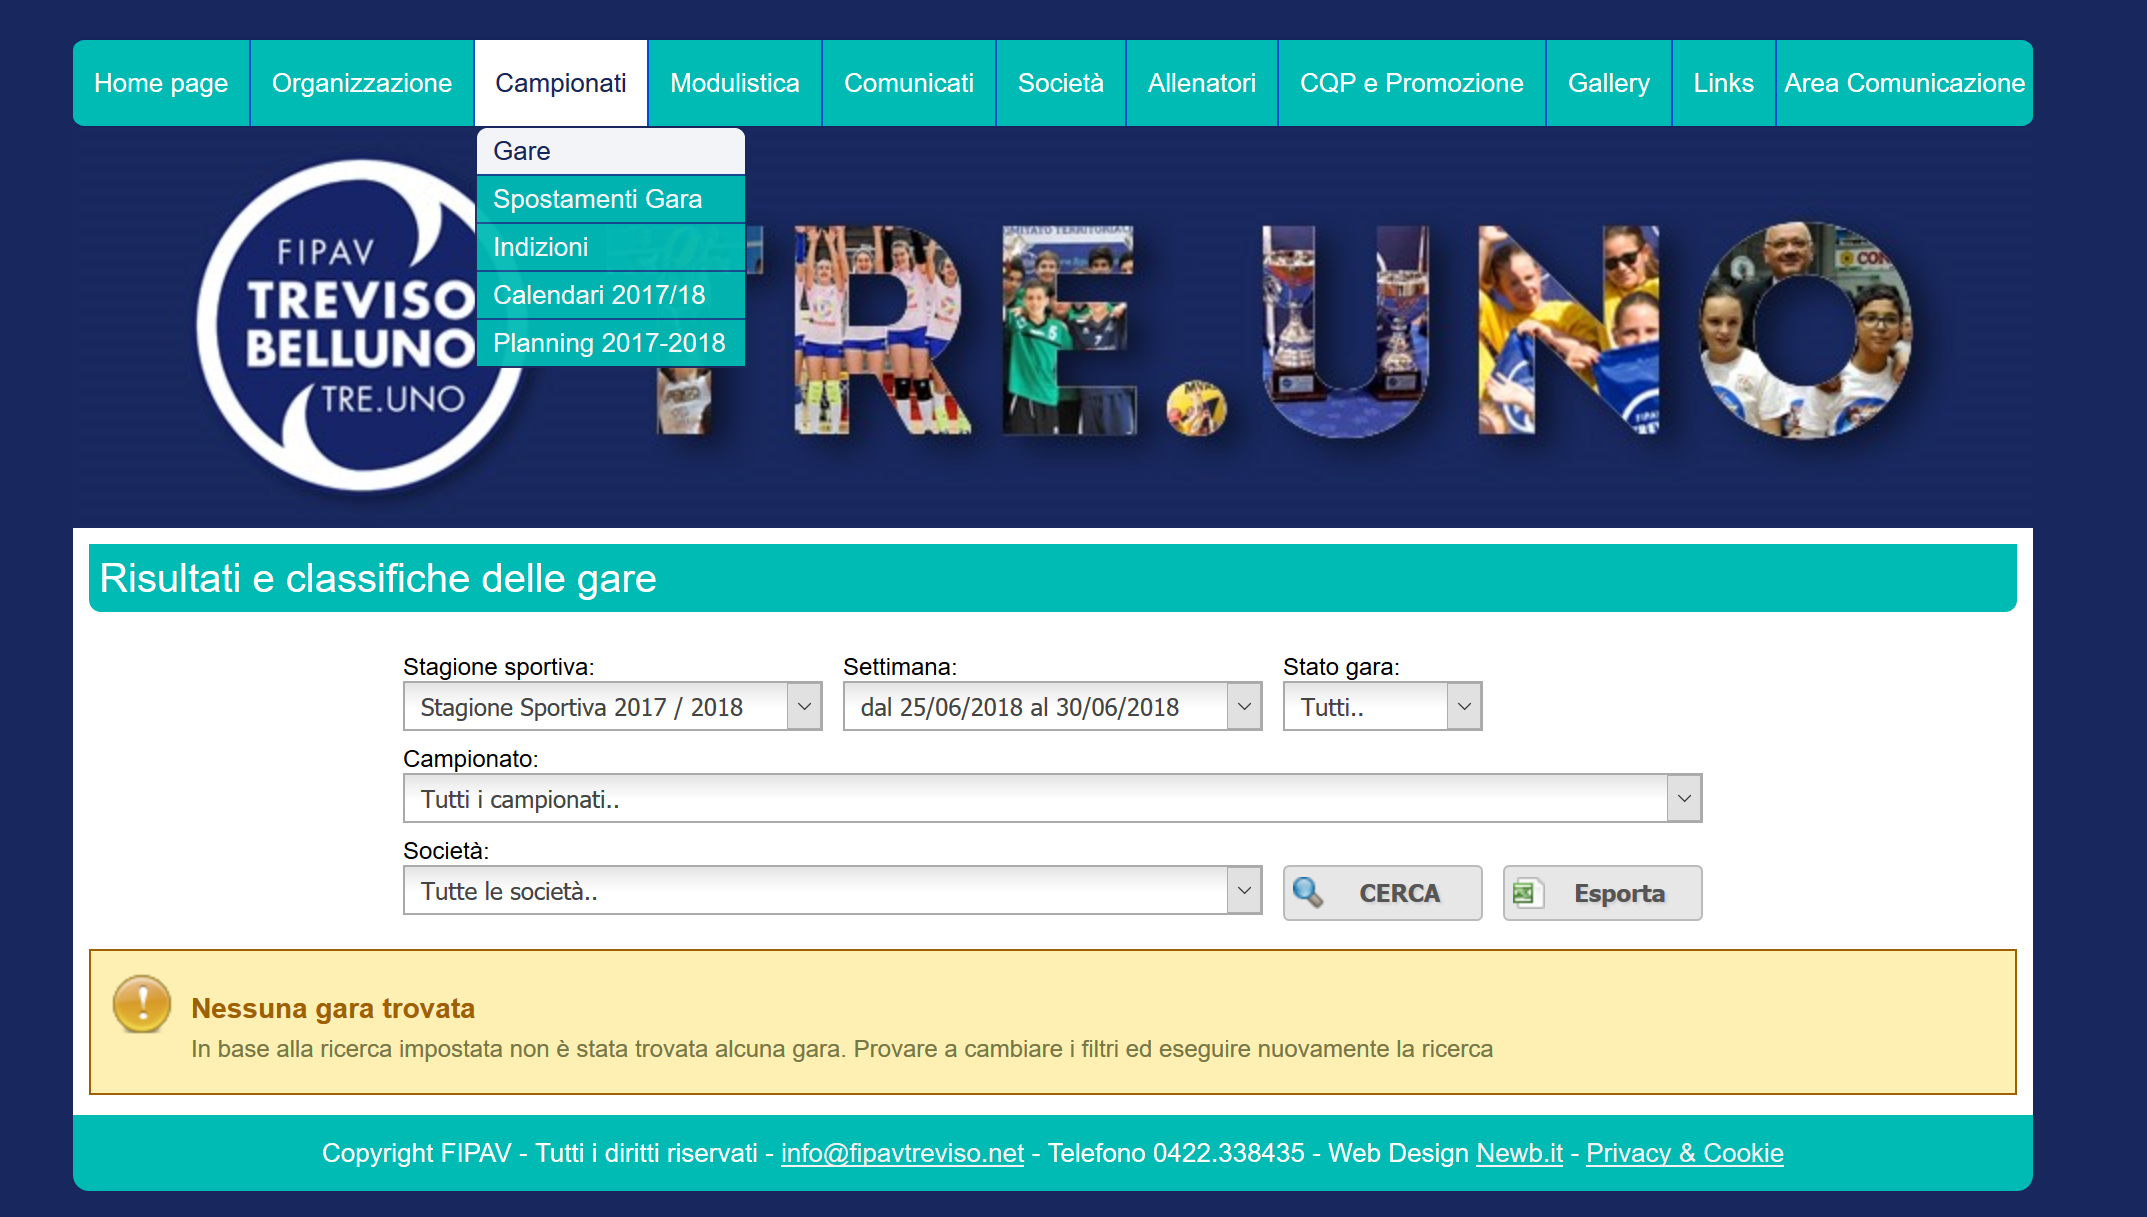
\includegraphics[scale=0.6]{Images/ricerca.png}
	\caption{Ricerca con filtri nella pagina \textit{Gare}}
	\end{figure}
	
	Infatti, quasi tutte le pagine presentano una lista, spesso molto lunga, di 
	informazioni senza dare all'utente uno strumento mirato per velocizzarne la 
	ricerca. Per esempio, nella pagina \textit{Società} viene illustrato una tabella 
	che necessità di circa 4 scroll per scorrerla tutta e non viene data la
	possibilità di ricercare una società specifica in modo più semplice.
	
	\begin{figure}[H]
	\centering
	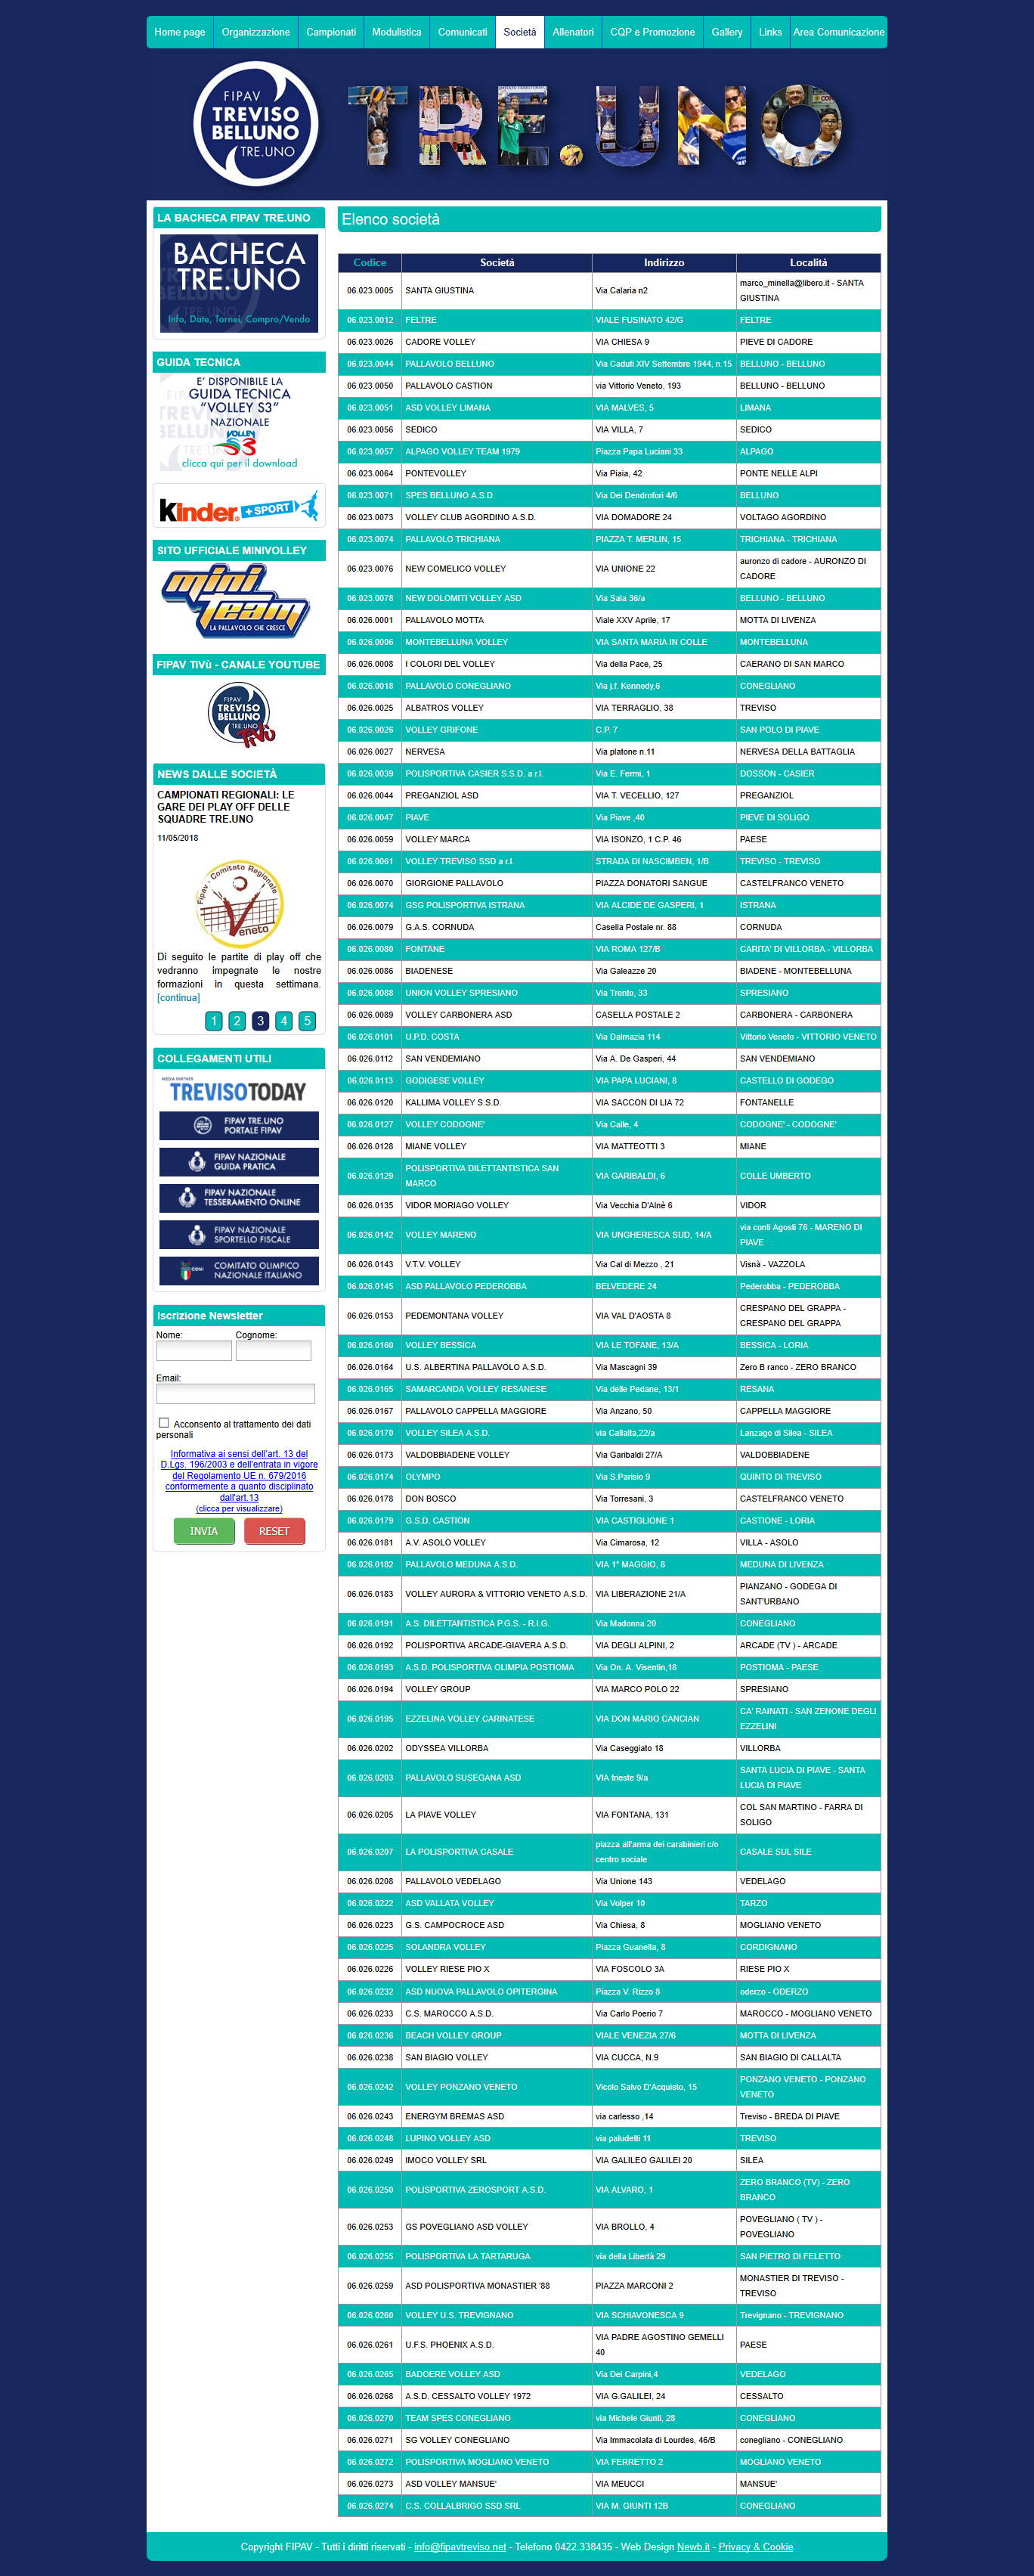
\includegraphics[scale=0.15]{Images/societa.png}
	\caption{Lista delle società nella pagina \textit{Società}}
	\end{figure}
	
	Ci sono però delle pagine che presentano sì queste lunghe liste, ma sono dotate 
	anche di una barra di ricerca così da non costringere l'utente, nei peggiori
	dei casi, a scorrere tutta la pagina prima di trovare ciò che cerca.
	Una di queste pagine è \textit{Archivio News} raggiungibile tramite 
	\textit{Area comunicazione}. Essa, infatti, presenta fin da subito una barra di
	ricerca per rintracciare con più facilità la notizia che interessa lasciando 
	comunque la possibilità di scorrerle tutte. Da notare che in questo caso, si è
	scelto di non creare una pagina lunghissima da scorrerla con un numero cospicuo 
	di scroll, ma di suddividere le notizie in pagine, così da rendere più facile 
	lo scorrimento di esse. Non è noto il motivo per cui solo in questa pagina le 
	informazioni siano state disposte in questo ordine, ma utilizzare questa 
	struttura anche nelle altre pagine, renderebbe il sito più usabile.
	
	\begin{figure}[H]
	\centering
	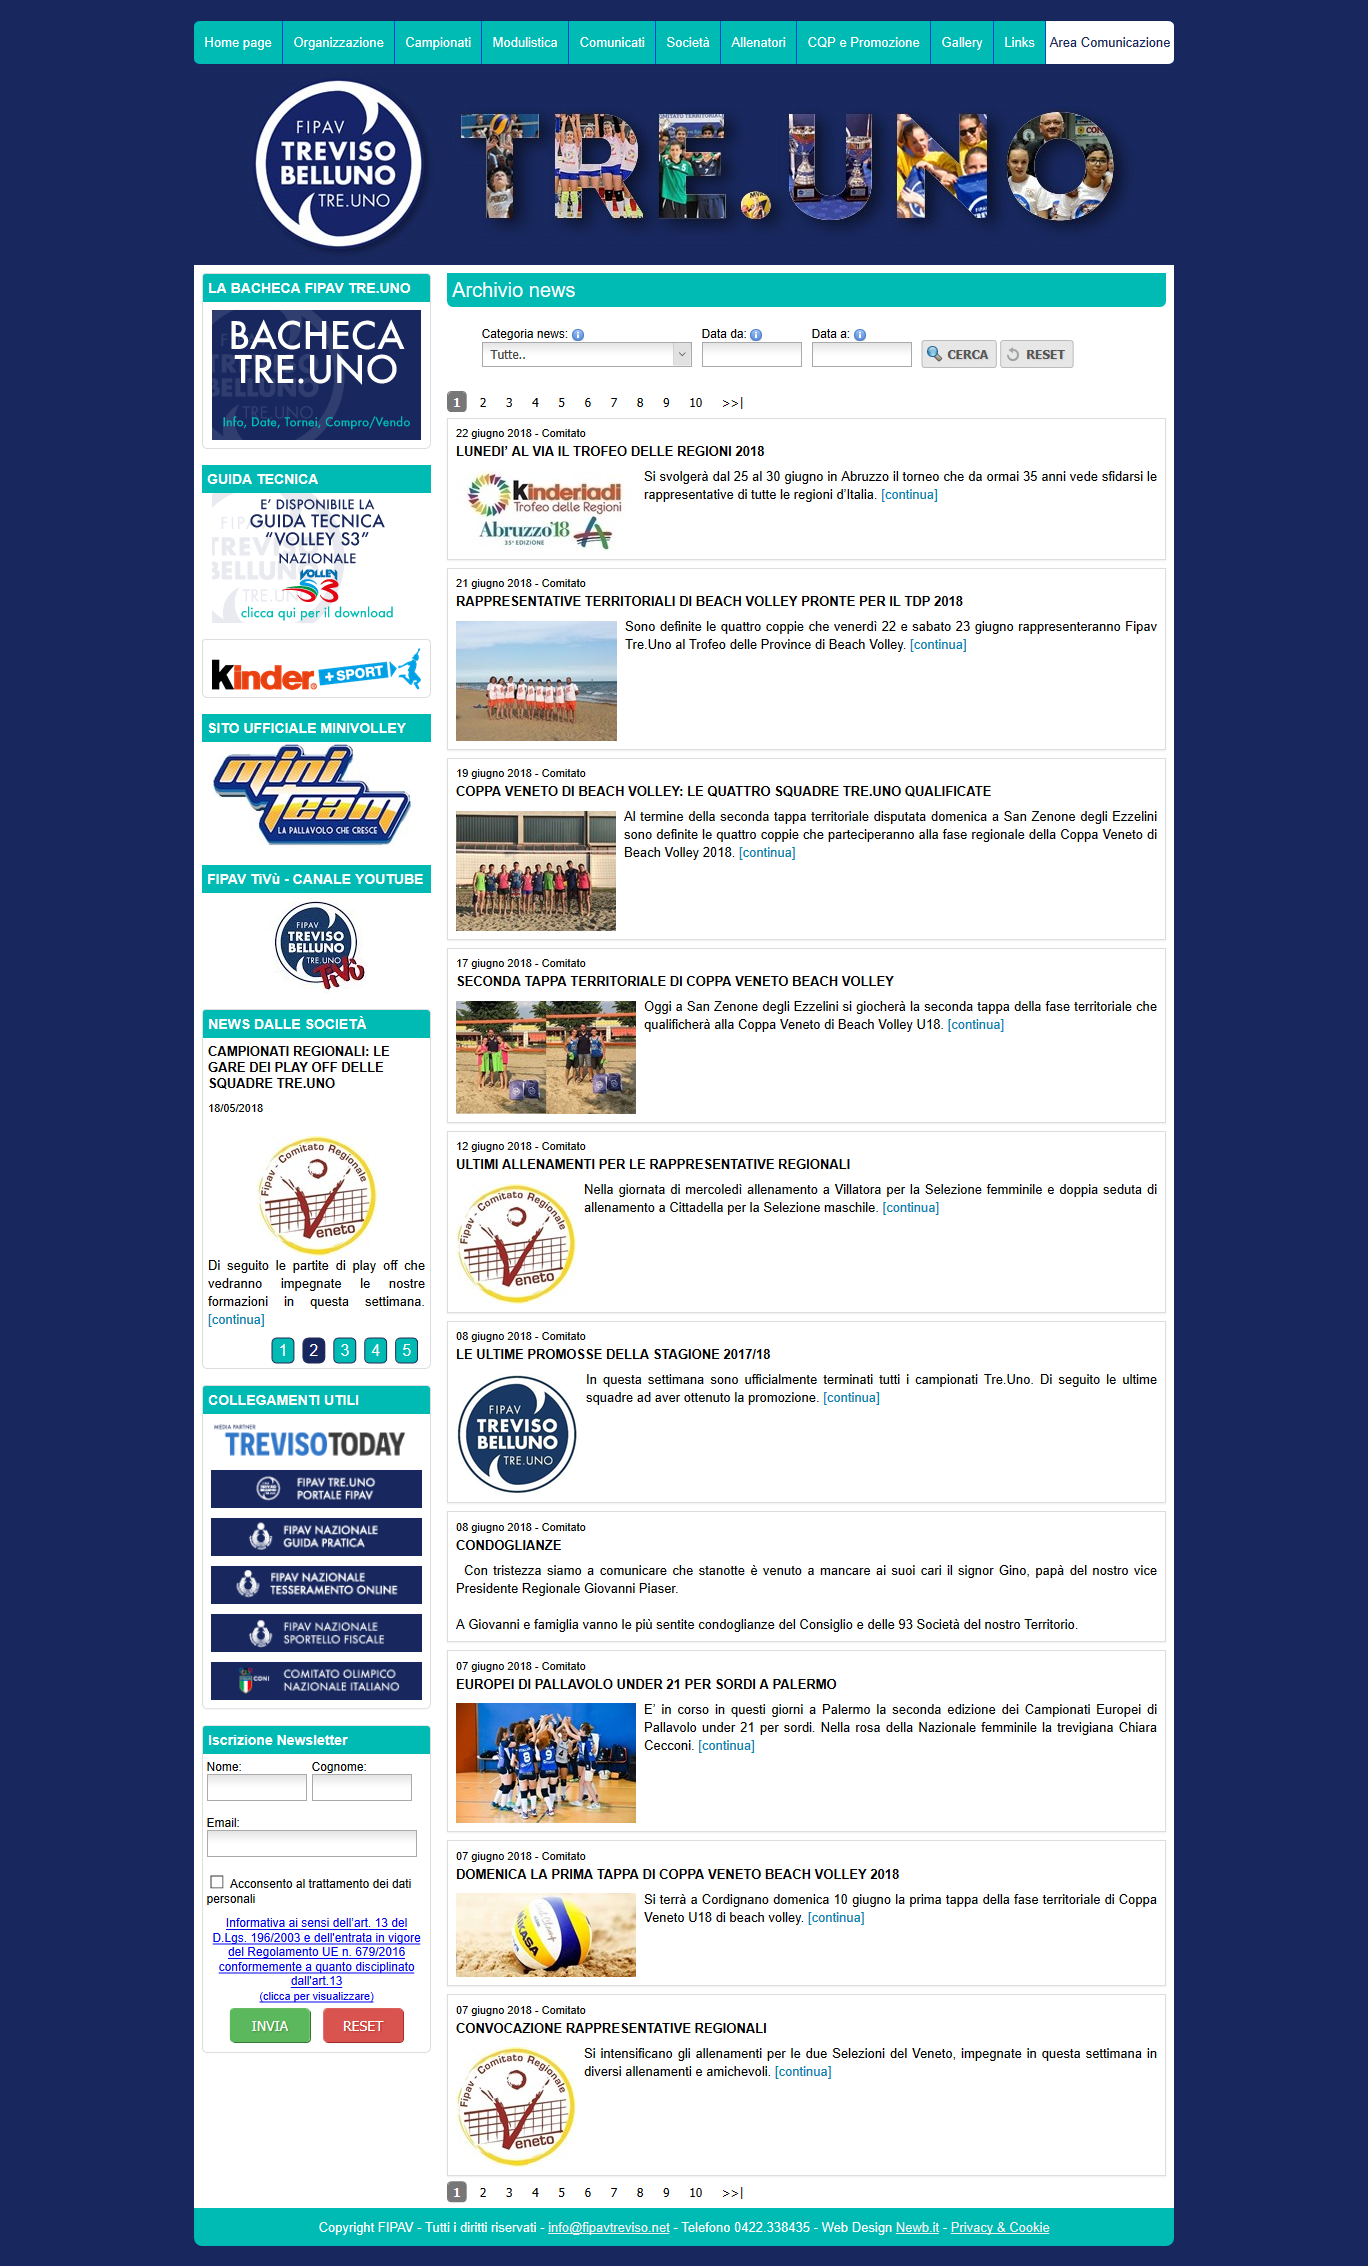
\includegraphics[scale=0.15]{Images/archivio.png}
	\caption{Lista delle news nella pagina \textit{Archivio News}}
	\end{figure}
	
	\subsection{Considerazioni generali}
	Essendo tali pagine praticamente uguali alla homepage se non per i contenuti e 
	il modo in cui vengono disposti come precedentemente spiegato, tutte le
	considerazioni fatte sulla homepage valgono anche per tali pagine. L'unica nota
	aggiuntiva da fare riguarda i breadcrumbs di tipo location: infatti questi non 
	sono presenti e per indicare all'utente in che pagina interna si trova, questa 
	viene evidenziata (e così succede se si accede a una pagina ancora più interna).
	
	\begin{figure}[H]
	\centering
	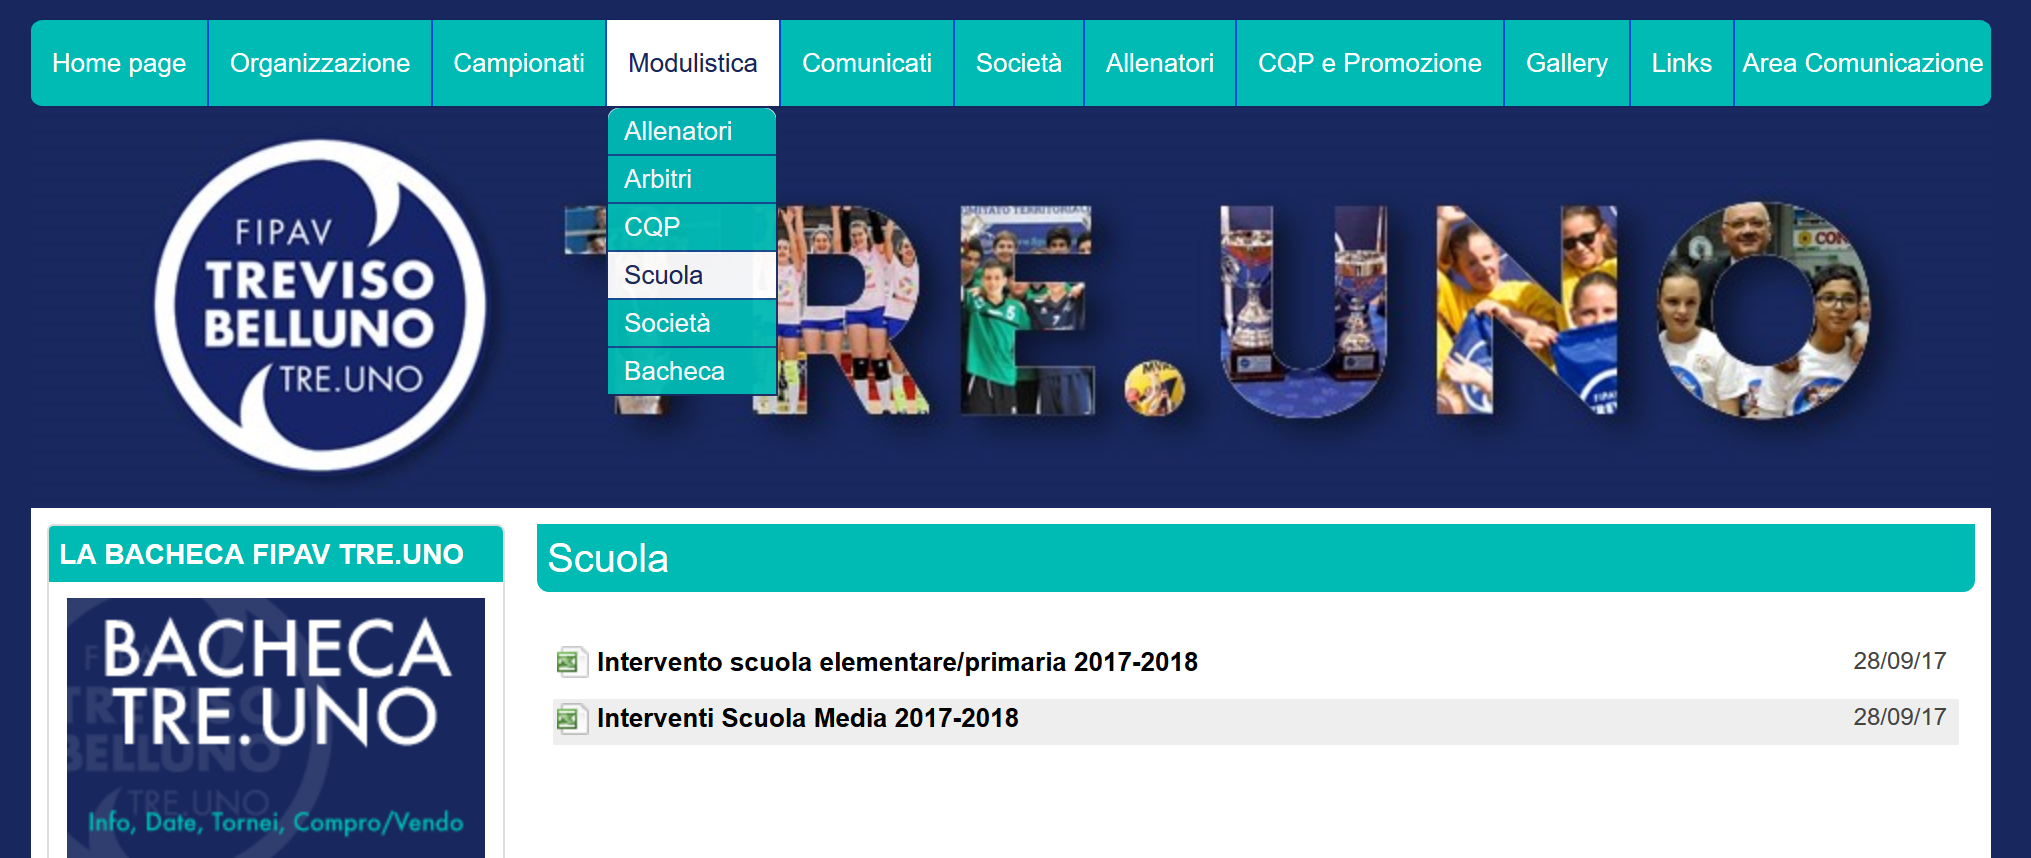
\includegraphics[scale=0.5]{Images/breadcrumb.png}
	\caption{Menù evidenziato sulla pagina interna scelta}
	\end{figure}
	
	Evidenziando comunque in che pagina ci si trova è possibile identificare 
	l'asse where, ma non viene usato nessun marcatore per ricordare all'utente che
	pagine ha già visitato.
	
	
	